\documentclass[conference]{IEEEtran}
\IEEEoverridecommandlockouts
% The preceding line is only needed to identify funding in the first footnote. If that is unneeded, please comment it out.
\usepackage{cite}
\usepackage{amsmath,amssymb,amsfonts}
\usepackage{algorithmic}
\usepackage{graphicx}
\usepackage{textcomp}
\usepackage{xcolor}

\def\BibTeX{{\rm B\kern-.05em{\sc i\kern-.025em b}\kern-.08em
    T\kern-.1667em\lower.7ex\hbox{E}\kern-.125emX}}
\begin{document}

\title{Experimental Bolus Sensor for Dairy Cattle\\
\thanks{Identify applicable funding agency here. If none, delete this.}
}

\author{\IEEEauthorblockN{Éva Nagyné Hajnal}
\IEEEauthorblockA{\textit{Alba Regia Technical Faculty} \\
\textit{Óbuda University}\\
Székesfehérvár, Hungary \\
email address or ORCID}
\and
\IEEEauthorblockN{Gergely Vakulya}
\IEEEauthorblockA{\textit{Alba Regia Technical Faculty} \\
\textit{Óbuda University}\\
Székesfehérvár, Hungary \\
email address or ORCID}
\and
\IEEEauthorblockN{Péter Udvardy}
\IEEEauthorblockA{\textit{Alba Regia Technical Faculty} \\
\textit{Óbuda University}\\
Székesfehérvár, Hungary \\
email address or ORCID}
}

\maketitle

\begin{abstract}
Abstract
\end{abstract}

\begin{IEEEkeywords}
dairy cattle, bolus, accelerometer
\end{IEEEkeywords}

\section{Introduction}

A great challenge of today's humanity is to serve the intensively
increasing demand for food, in an environmentally friendly manner.
A promising way to address this problem is precision agriculture,
based on extensive monitoring. In our research we focus on dairy
cattle and rumen bolus sensors. This paper presents the preliminary
results of an experimental bolus, equipped with accelerometer,
shock sensor and temperature meter.


%\begin{table}[htbp]
%\caption{Table Type Styles}
%\begin{center}
%\begin{tabular}{|c|c|c|c|}
%\hline
%\textbf{Table}&\multicolumn{3}{|c|}{\textbf{Table Column Head}} \\
%\cline{2-4} 
%\textbf{Head} & \textbf{\textit{Table column subhead}}& \textbf{\textit{Subhead}}& \textbf{\textit{Subhead}} \\
%\hline
%copy& More table copy$^{\mathrm{a}}$& &  \\
%\hline
%\multicolumn{4}{l}{$^{\mathrm{a}}$Sample of a Table footnote.}
%\end{tabular}
%\label{tab1}
%\end{center}
%\end{table}

\section{Measurement environment}

TODO


\section{Measurement setup}

\subsection{Bolus sensor}

Design of the bolus is constrained by several factors. As these type
of devices are getting more and more standard, special applicators are
exist to inject them into the rumen. The physical dimensions are therefore
limited by the applicator. The desired form factor is a cylinder with
diameter of 40 mm and length of 140 mm.

The material of the bolus should resist the environment inside the rumen,
i.e. the moisture, temperature, motion and pH. The cover should protect
the sensitive electronics inside sensor. The POM-C technical plastic was
chosen as the material, which can be easily machined on a lathe and provides
the required strength and sealing.

A more or less fixed orientation of the bolus would ease the signal
processing of the accelerometer. To provide some defined orientation
in at least one axis the weight distribution of the bolus is designed
to be asymmetrical, the battery being one one end and a low density
material on the other side. The electronics are placed in between these two.

\begin{figure}[htbp]
\centerline{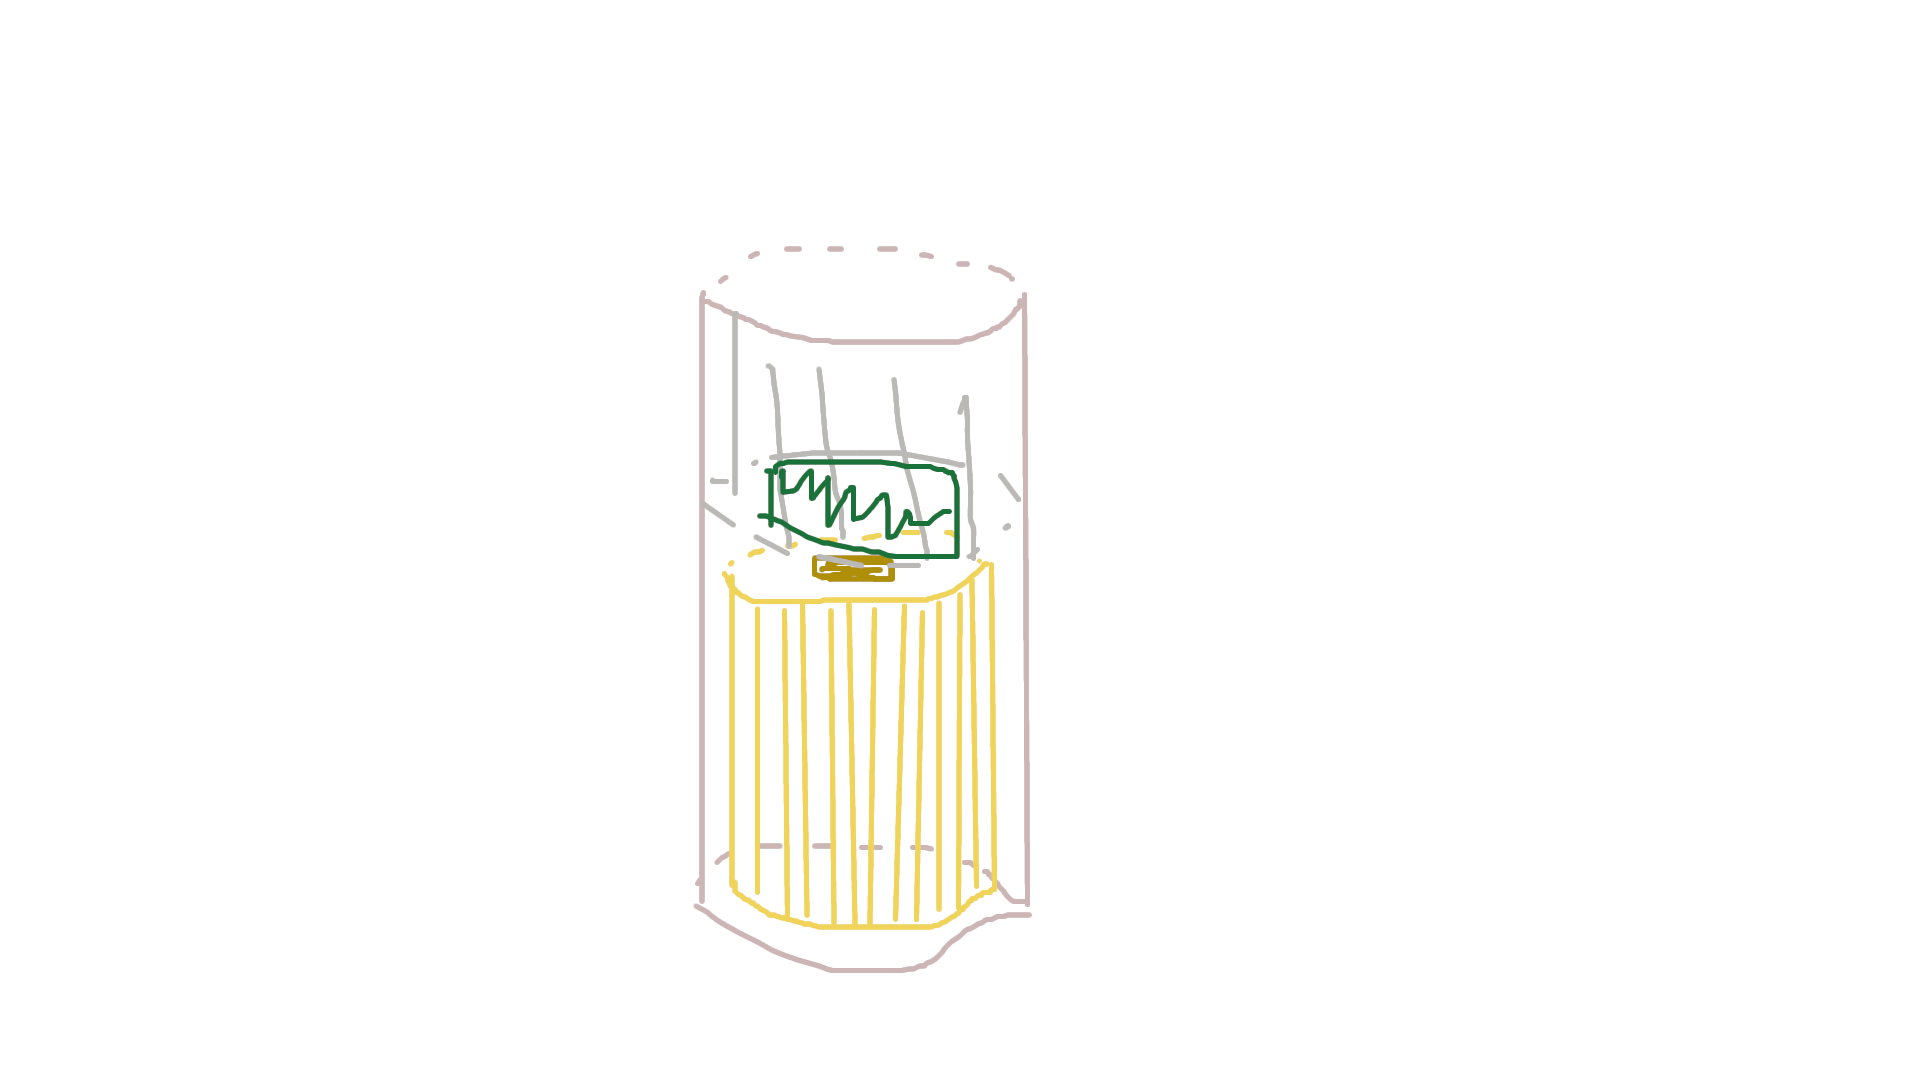
\includegraphics[width=0.35\textwidth]{fig/bolus-physical-layout.png}}
\caption{The physical layout of the bolus.}
\label{bolus-physical-layout}
\end{figure}

The physical layout of the bolus is shown in Fig. \ref{bolus-physical-layout}.


\begin{figure}[htbp]
\centerline{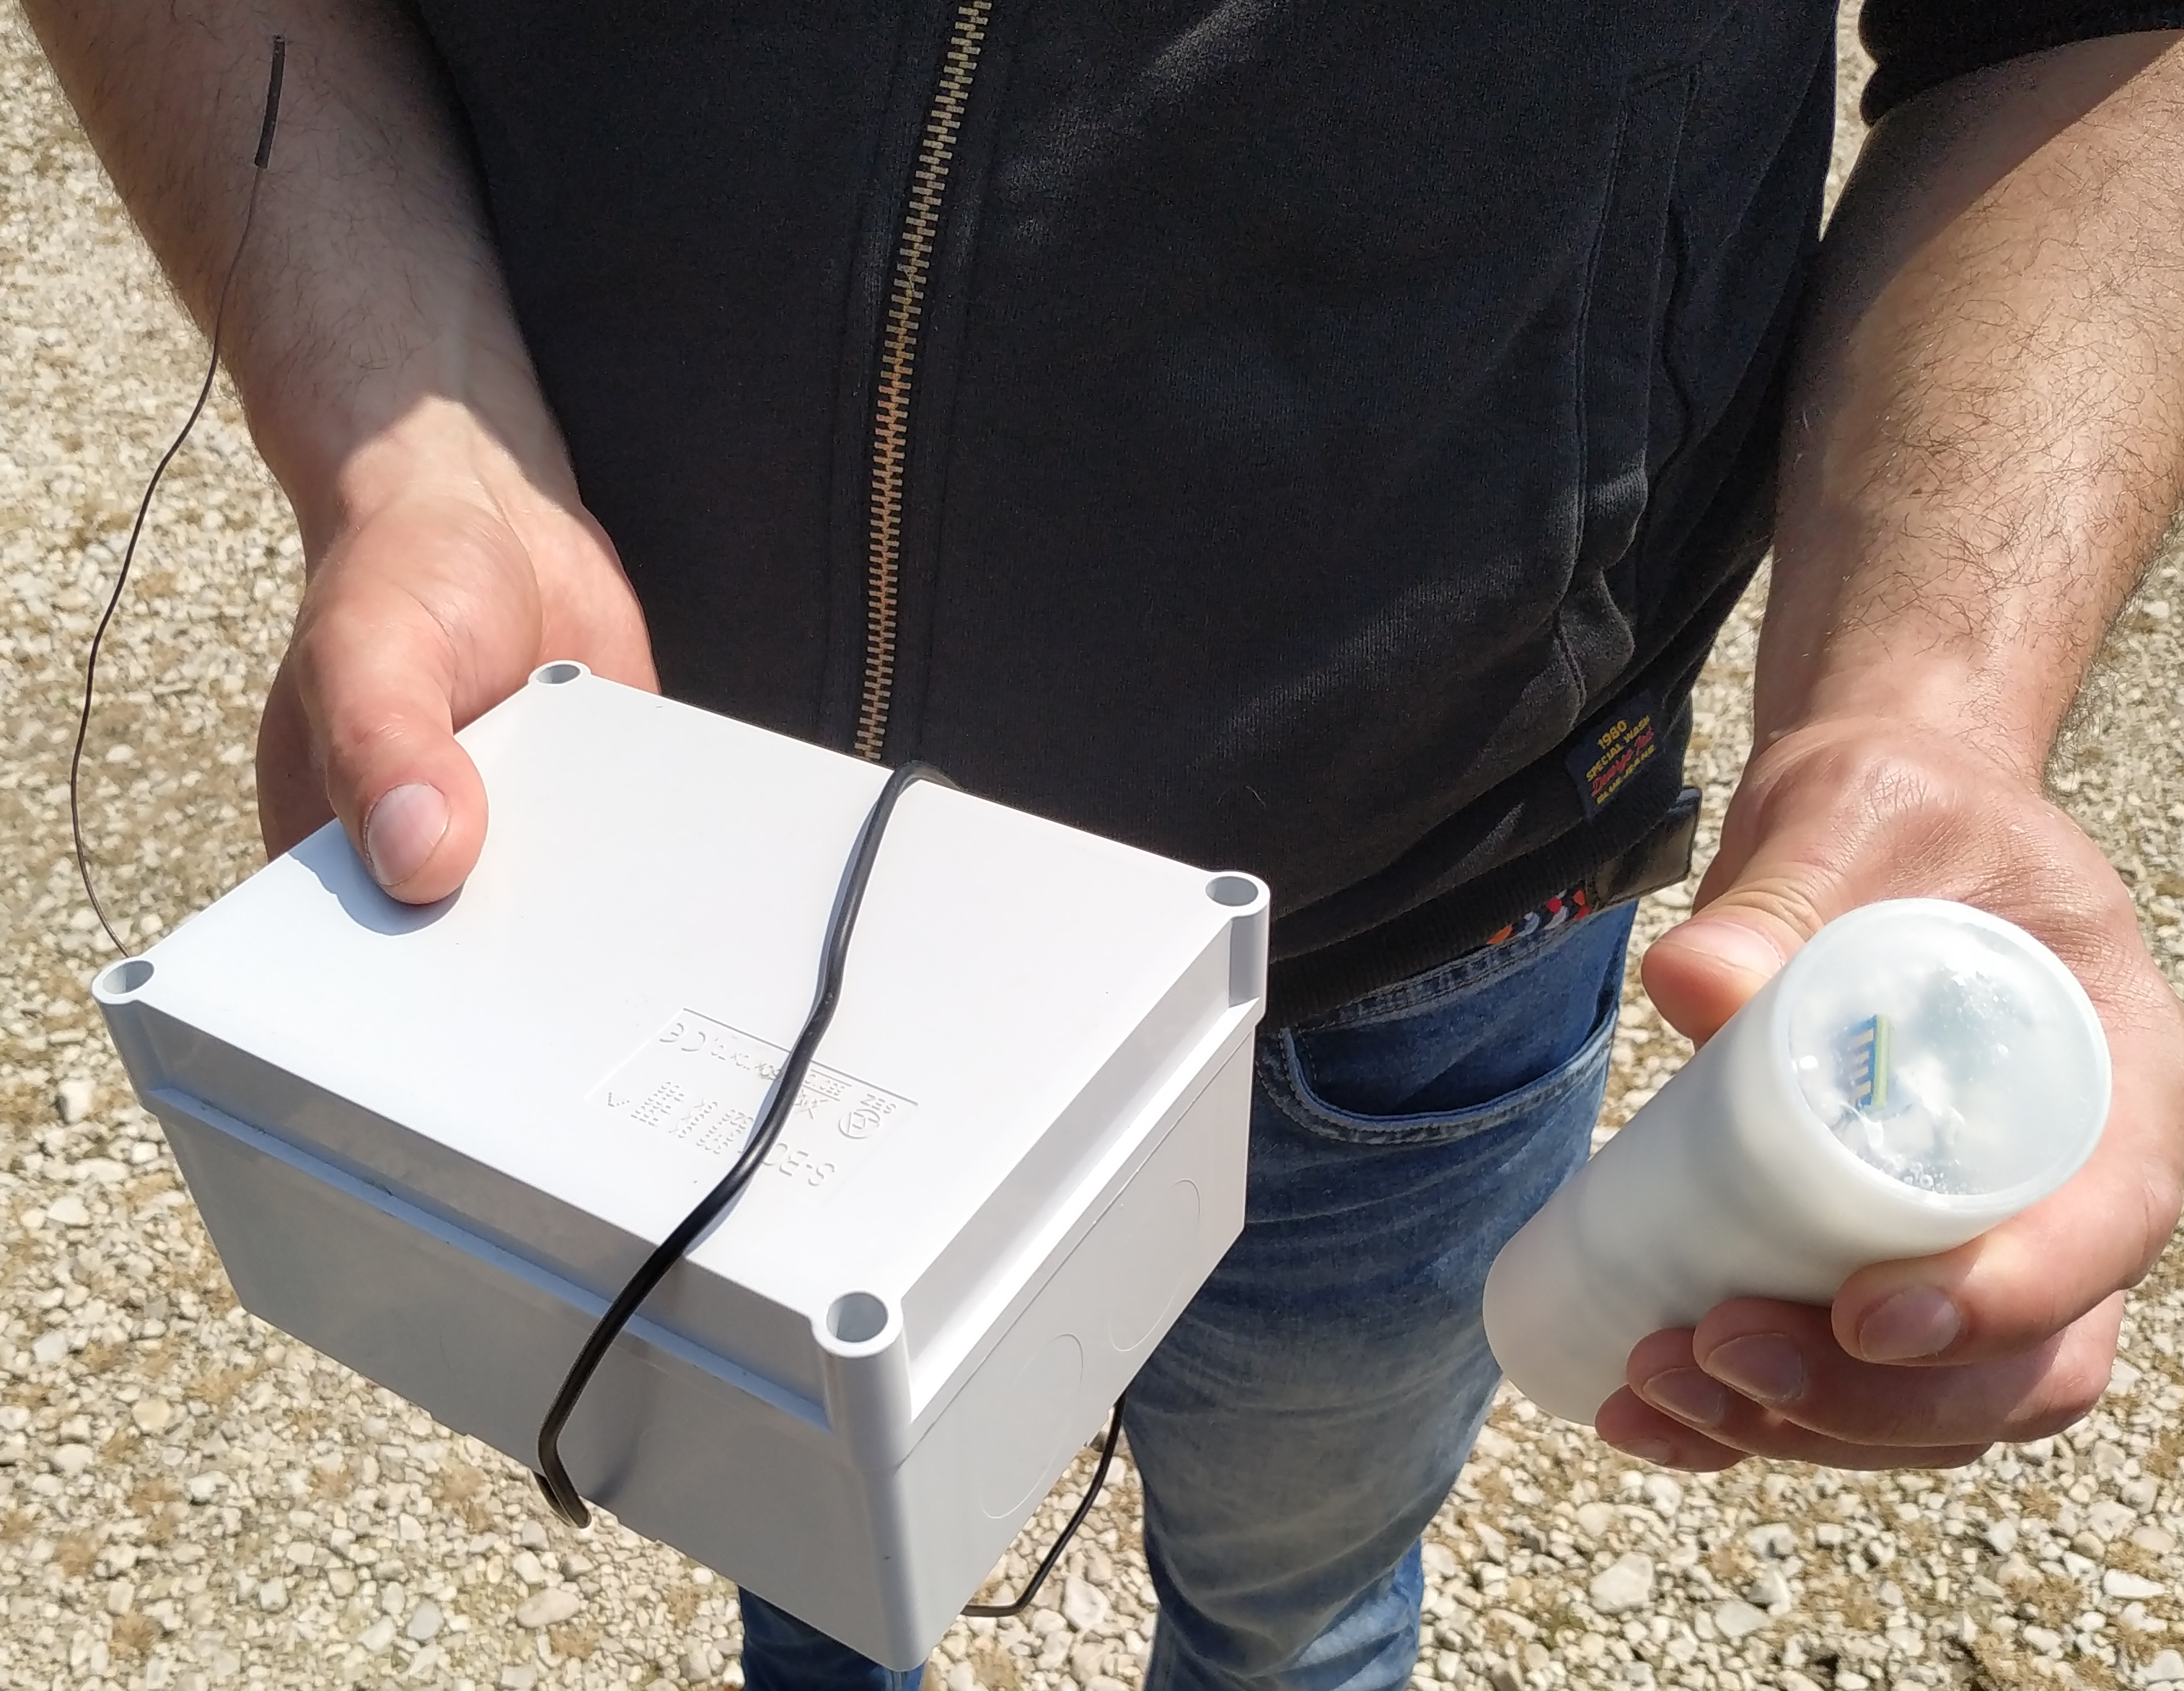
\includegraphics[width=0.35\textwidth]{fig/bolus_gw_photo.jpg}}
  \caption{The bolus (right side) and the gateway (left side).}
\label{bolus-gw-photo}
\end{figure}

Physical design

\begin{figure}[htbp]
\centerline{
  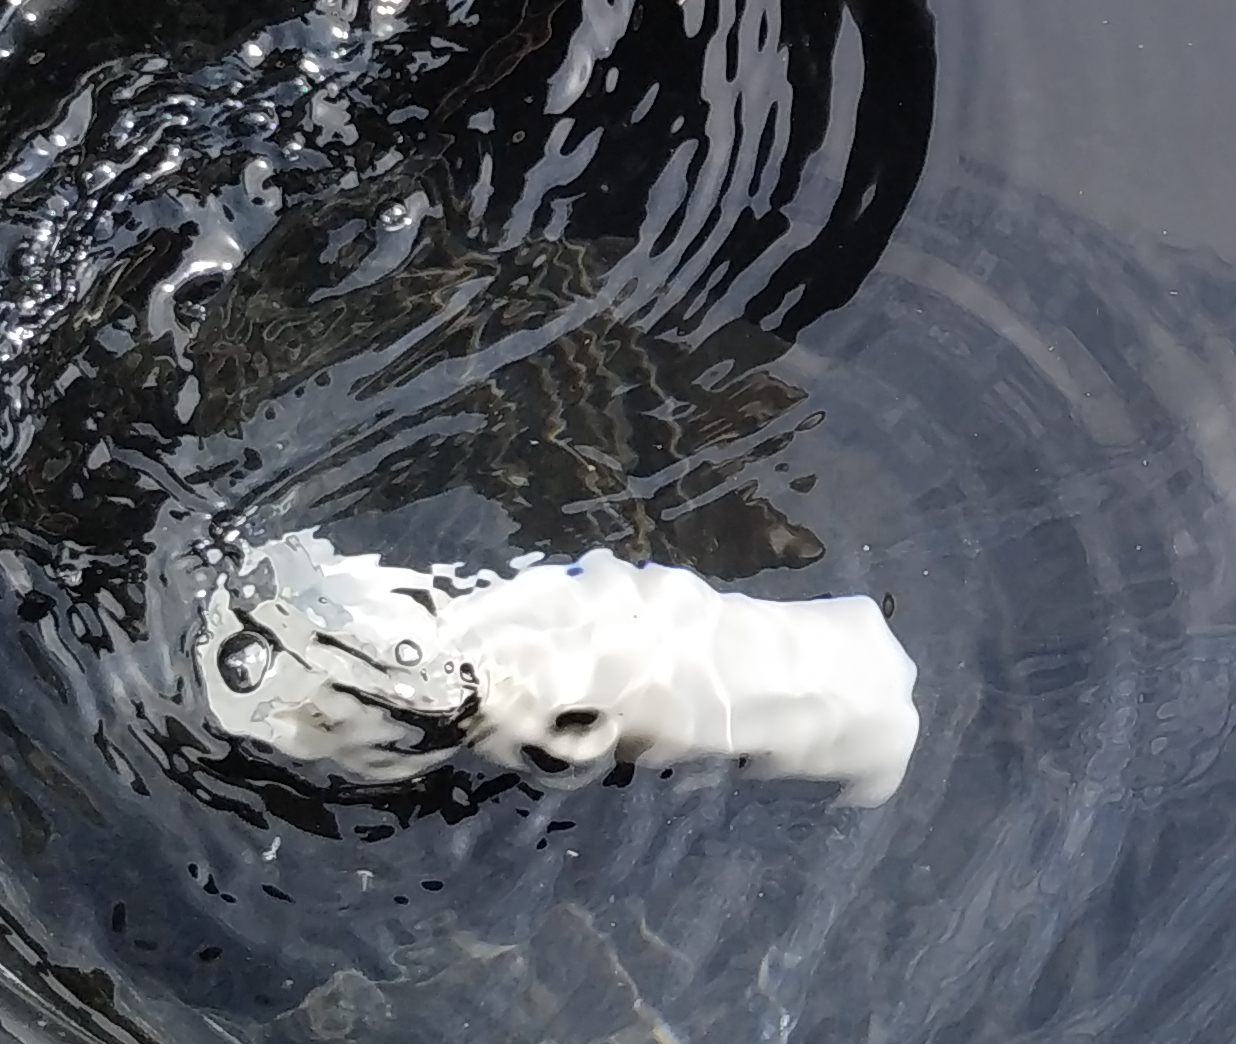
\includegraphics[width=0.15\textwidth]{fig/kfj_1.png}
  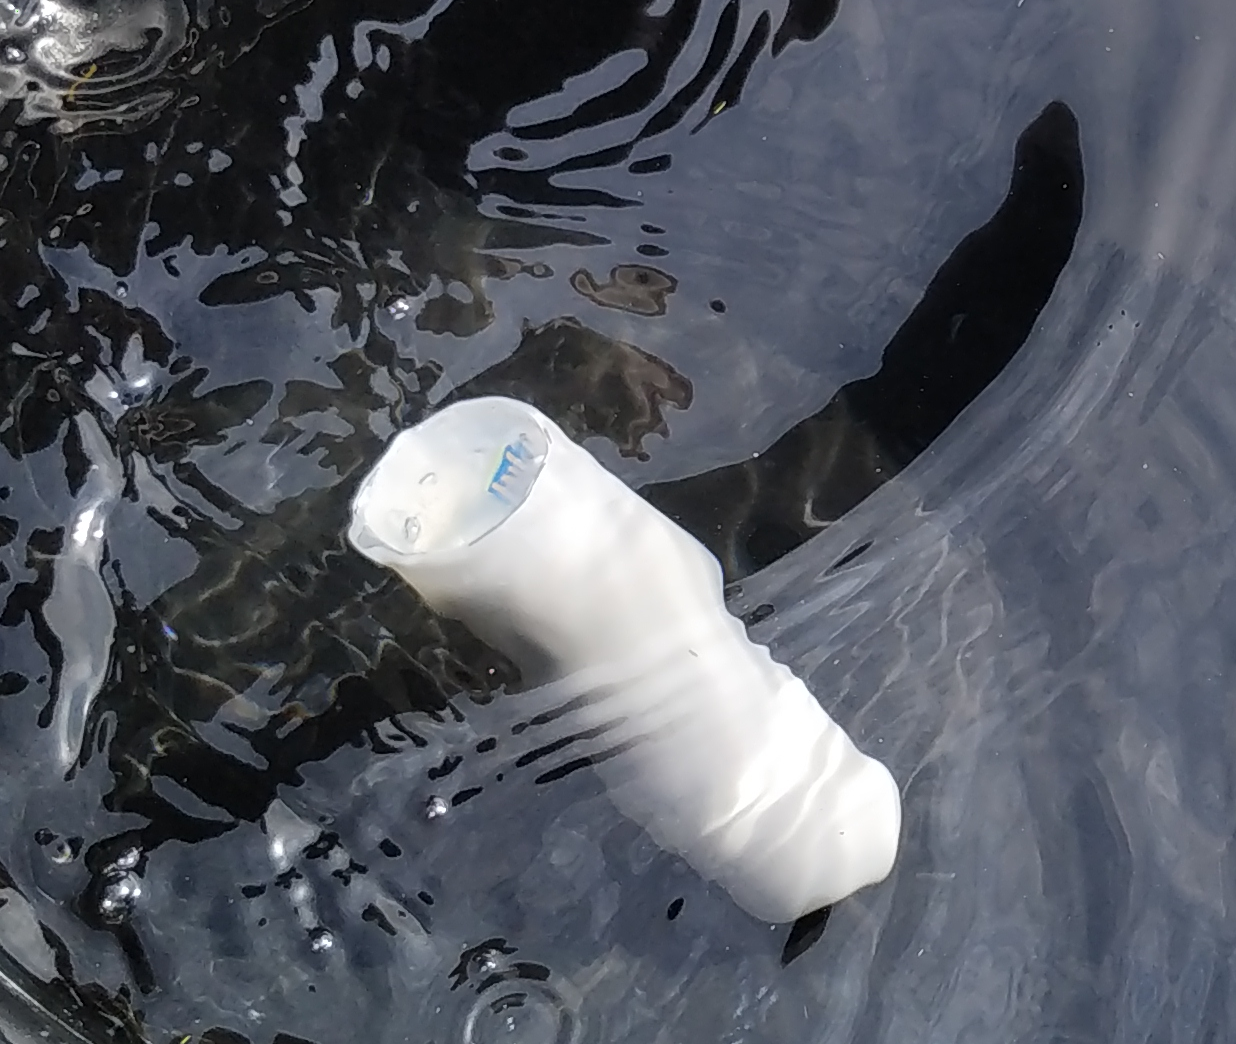
\includegraphics[width=0.15\textwidth]{fig/kfj_2.png}
  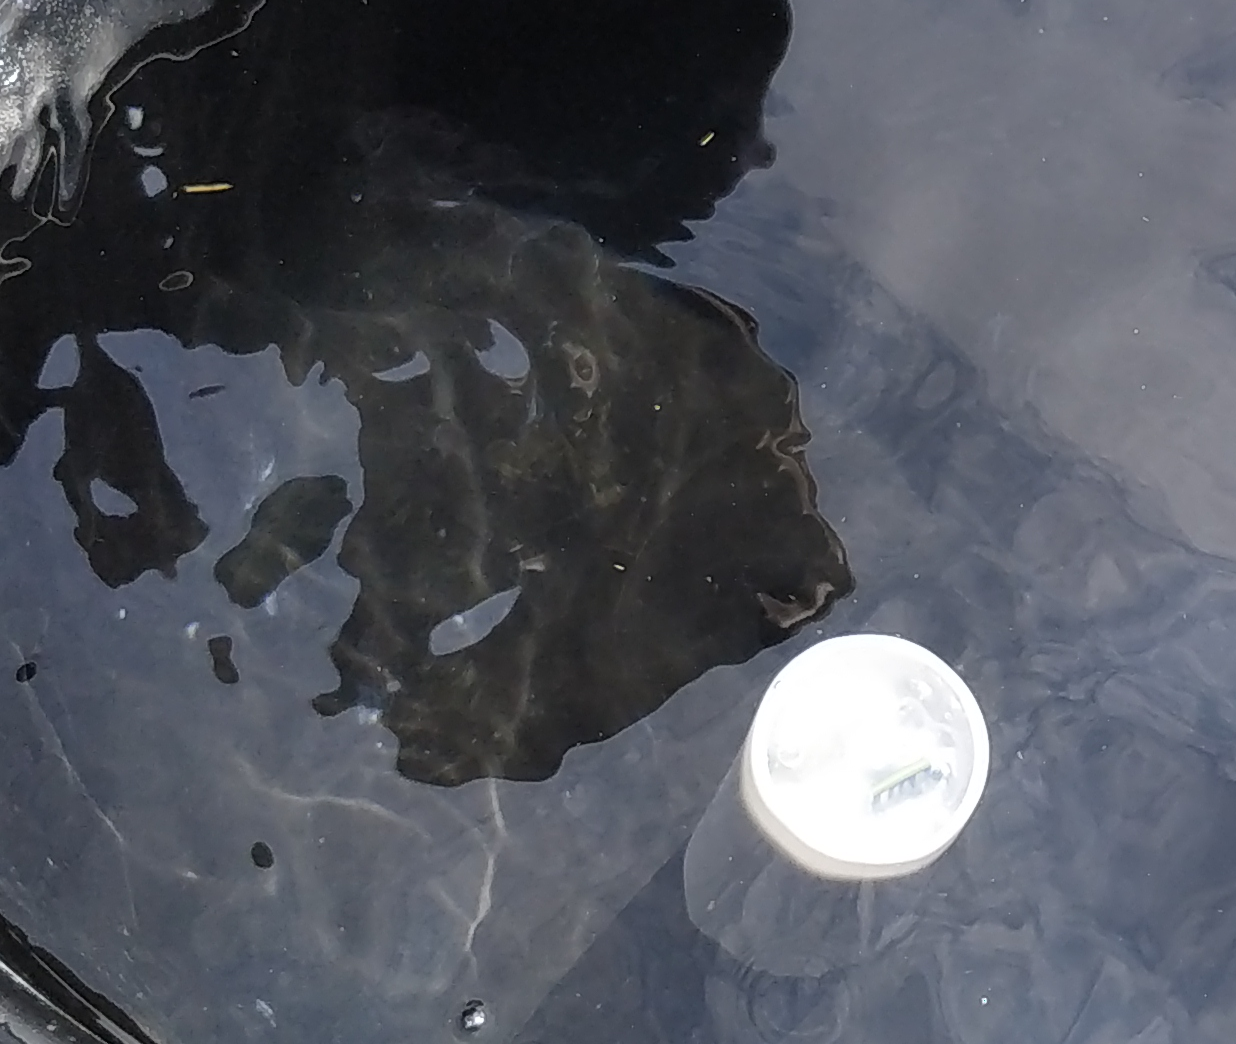
\includegraphics[width=0.15\textwidth]{fig/kfj_3.png}
  }
  \caption{Experiment of the self-orientation of the bolus sensor. The
  bolus is placed in a horizontal position in water (left side), then takes
  an upright position (middle, then right side).}
\label{bolus-gw-photo}
\end{figure}

\subsection{Gateways}

\subsection{Injecting the bolus}

\begin{figure}[htbp]
\centerline{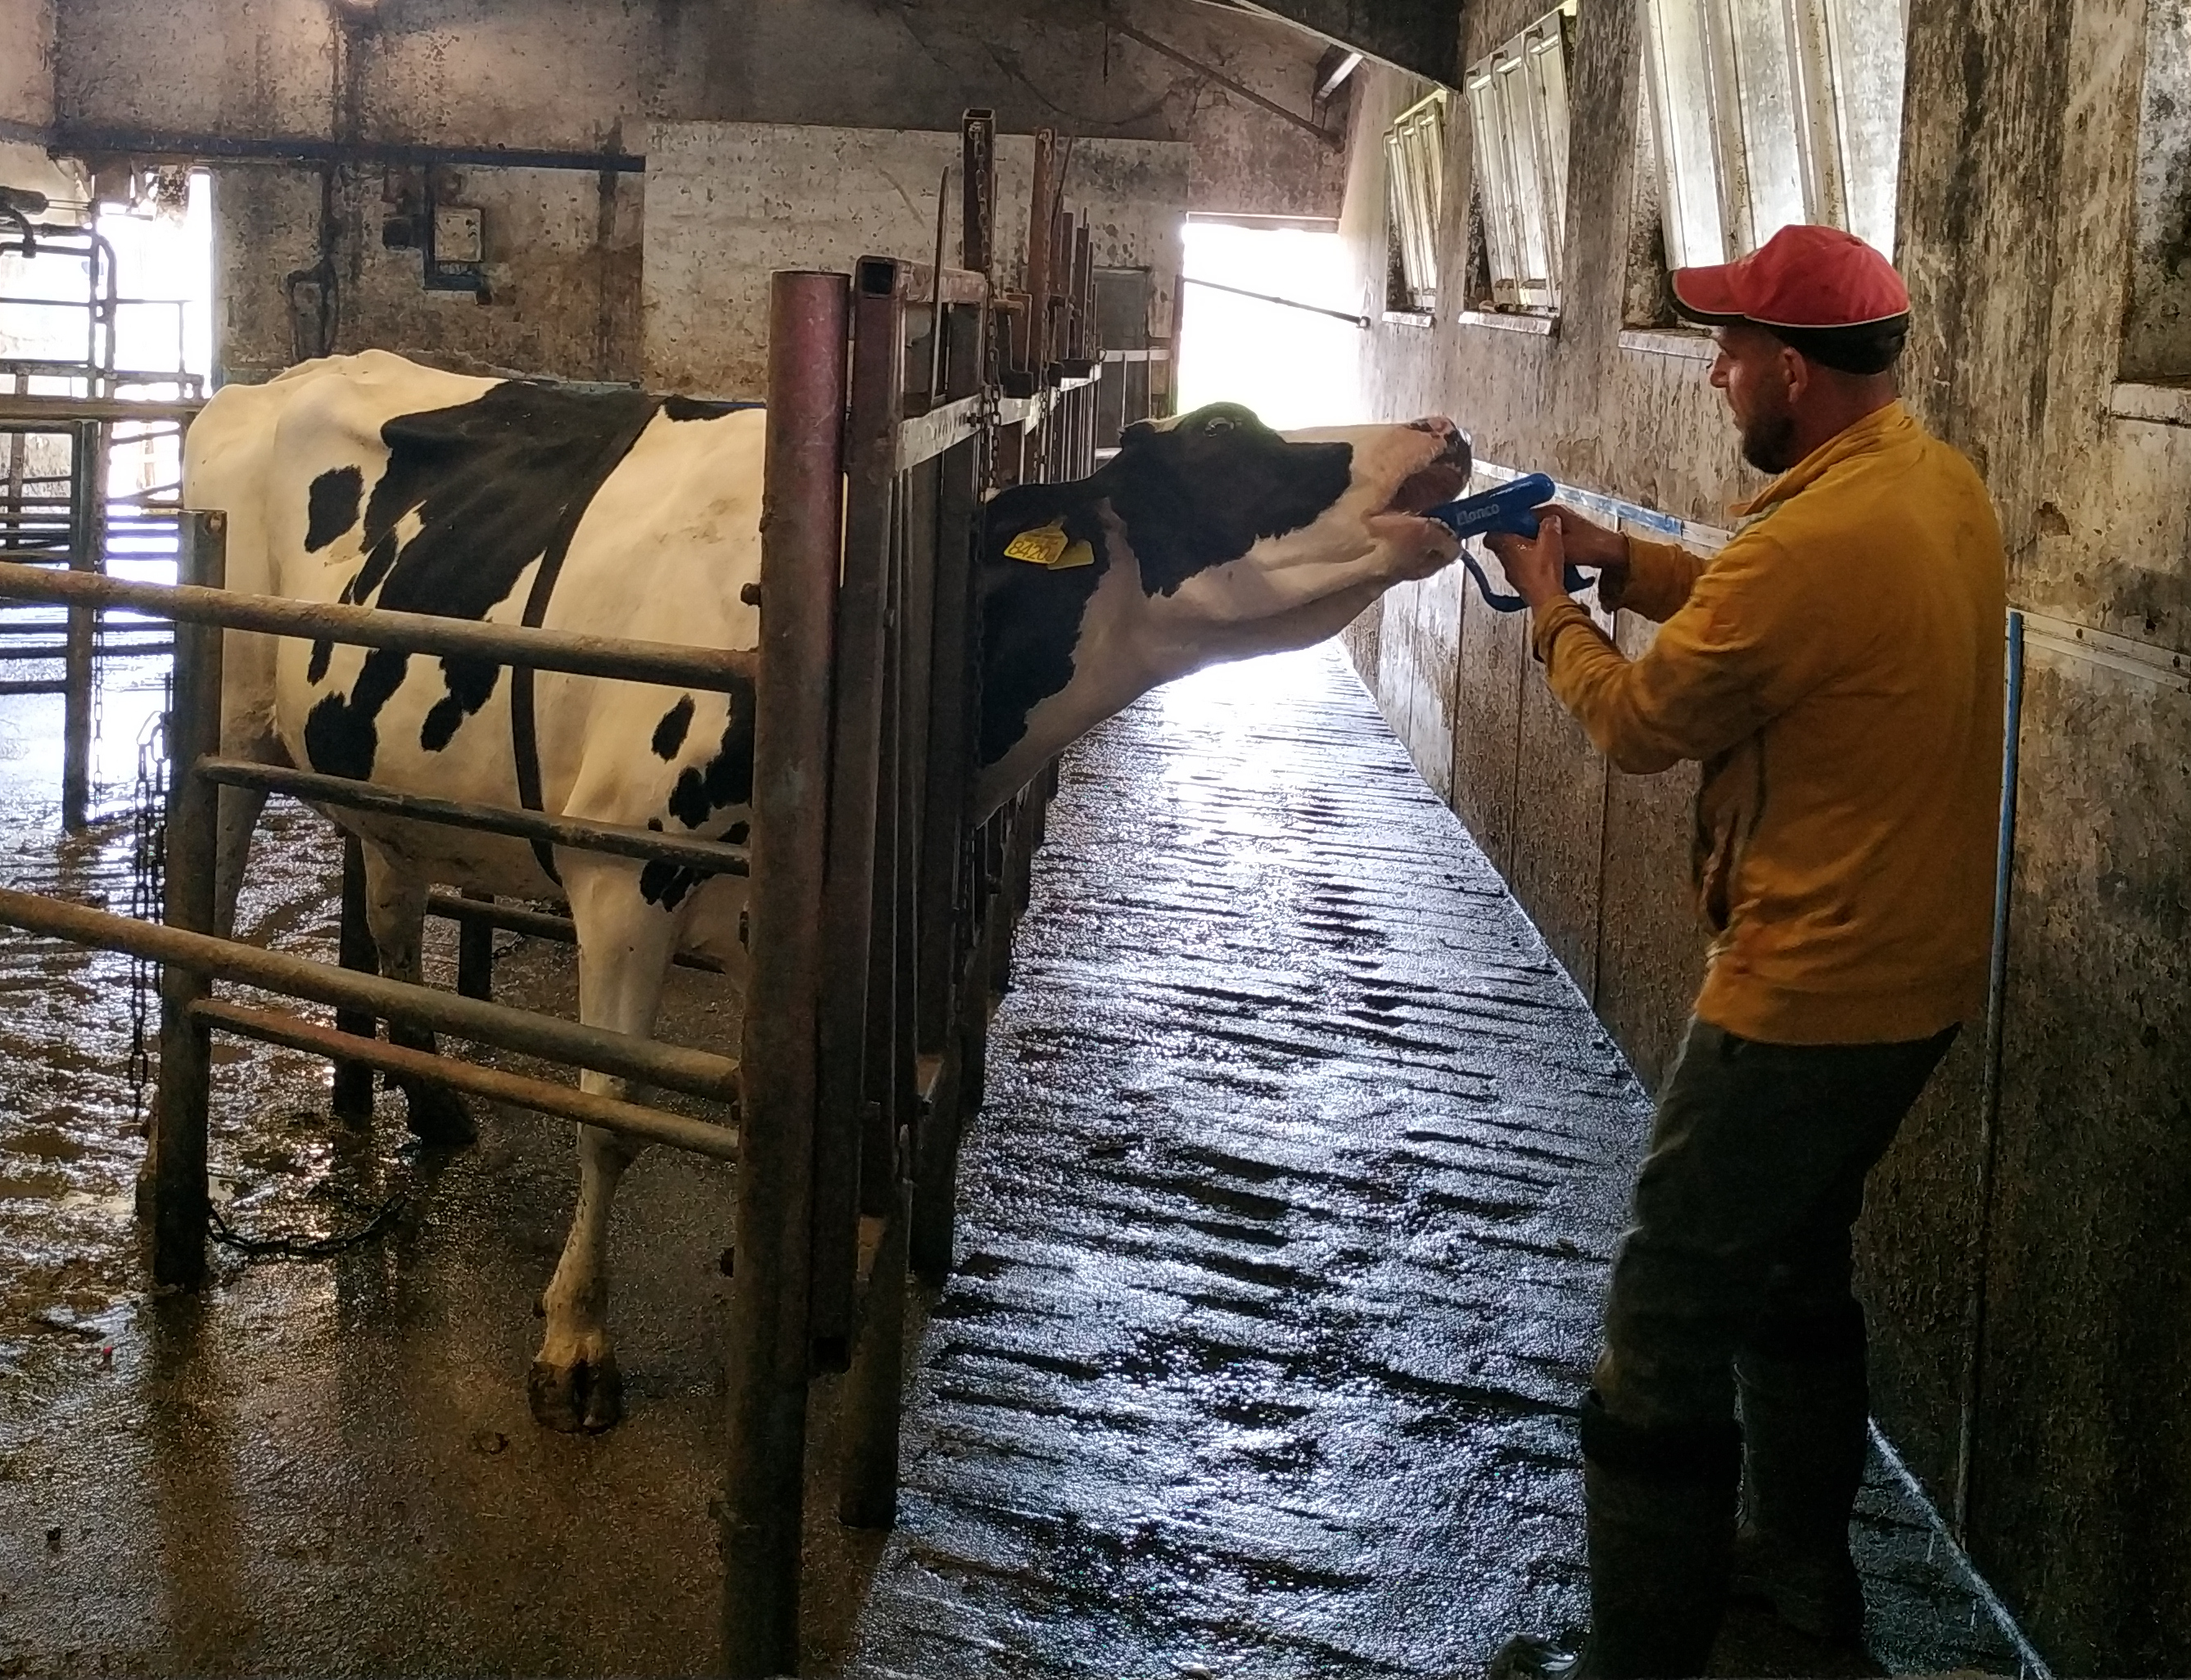
\includegraphics[width=0.35\textwidth]{fig/bolus_application.jpg}}
  \caption{Injecting the bolus with the applicator.}
\label{bolus-gw-photo}
\end{figure}


\subsection{Data format}


\section{Results}

\cite{nagl2003}

\section{Summary}

\section*{Acknowledgment}

The preferred spelling of the word ``acknowledgment'' in America is without 
an ``e'' after the ``g''. Avoid the stilted expression ``one of us (R. B. 
G.) thanks $\ldots$''. Instead, try ``R. B. G. thanks$\ldots$''. Put sponsor 
acknowledgments in the unnumbered footnote on the first page.

\bibliographystyle{IEEEtran}
\bibliography{IEEEabrv,references}

\end{document}
